\section{Problema 2: Sensores defectuosos}

\subsection{Introducci\'on}

\quad Se tiene un conjunto de sensores con sus respectivos intervalos de tiempo de medici\'on y se conoce el n\'umero de la medici\'on que falla. Se desea conocer el id del sensor que fall\'o. 

\subsection{Desarrollo}

\quad Encaramos este problema rearmando la secuencia de mediciones de los sensores. Consiguiendo \'esto, la soluci\'on al problema ser\'ia fijarse en esta secuencia, el id que figura en la posici\'on de medici\'on que fall\'o.


\quad Para armar la secuencia de mediciones, decidimos ir guardando para cada sensor en que instante de tiempo tendr\'ia que volver a realizar una medici\'on. A medida que determinamos el sensor que va a medir, calculamos su siguiente tiempo de medici\'on.


\quad Teniendo un diccionario donde para cada sensor se puede obtener en qu\'e momento le toca realizar una medici\'on, se puede conocer al pr\'oximo que le toca medir, ya que es el m\'inimo de los tiempos.


\quad En el momento inicial todos los sensores miden, por lo que la secuencia inicial no es vac\'ia, sino que contiene todos los n\'umeros de sensores ordenados por su id ya que desempatan por \'este.


\quad En cada paso de nuestro algoritmo, agregamos a la secuencia el siguiente sensor que midi\'o y calculamos su pr\'oxima medici\'on actualizando la tabla de pr\'oximas mediciones


\quad Cuando la secuencia alcanza el tama\~no igual al n\'umero de medici\'on que fall\'o, terminamos y el resultado es la \'ultima posici\'on de esa secuencia.

\quad

\textbf{Aclaraci\'on:} en la implementaci\'on del diccionario se usa directamente un min-Heap. M\'as adelante se explica el motivo de tal decisi\'on.



\quad


\textbf{Pseudoc\'odigo:}

\begin{algorithm}[H]
\begin{algorithmic}[1]
\STATE Diccionario diccTiempos  \quad $ \gets $ \quad sensores
\STATE Entero medicion $ \gets \vert$ sensores $ \vert $
\FORALL{ Sensor s \textbf{in} sensores}
\STATE agregar(mediciones,id(s))
\ENDFOR
\WHILE{medicion < medDefectuosa}
\STATE proximo \quad $ \gets $ \quad proxSensor(diccTiempos,sensores)
\STATE agregar(mediciones,proximo)
\STATE medicion $ \gets $ medicion + 1
\ENDWHILE
\end{algorithmic}
\caption{Entero sensorDefectuoso(Conjunto sensores, Entero medDefectuosa)}\label{probConjK}
\end{algorithm}


\quad


\textbf{Donde}


\quad \quad \quad medDefectuosa es el n\'umero de medici\'on que falla.

\quad


\quad \quad \quad diccTiempos es el diccionario que para cada sensor guarda el tiempo de su pr\'oxima medici\'on.

\quad


\quad \quad \quad sensores es el conjunto de sensores.


\quad

\quad \quad \quad medicion es el n\'umero de medici\'on parcial. Como al inicio hubo la cantidad de sensores, se inicializa con esa cantidad.


\quad

\quad \quad \quad mediciones es la secuencia de mediciones con los ids de los sensores.


\quad

\quad \quad \quad proxSensor es la funcion que devuelve el id del m\'inimo de los tiempos que est\'an presentes en el diccionario, y adem\'as actualiza el tiempo para la pr\'oxima medici\'on.


\subsubsection{Correctitud}

\quad En alguna instancia del problema, si tuvi\'eramos la siguiente tabla con los momentos $ t_i $ para la siguiente medici\'on de cada sensor $ s_i $ con \quad  $ (1 \leq i \leq n)$ \quad donde n es la cantidad total de sensores:


\quad


\begin{tabular}{| c | c | c | c | c |}
\hline
$ s_1 $ & $ s_2 $ & ... & $ s_{n-1} $ & $ s_n $\\
\hline
$ t_1 $ & $ t_2 $ & ... & $ t_{n-1} $ & $ t_n $\\
\hline

\end{tabular}



\quad


\quad determinar el siguiente sensor que le toca realizar su medici\'on, ser\'ia elegir el de menor t. Caso contrario, se estar\'ia eligiendo un sensor con tiempo mayor, por lo que har\'ia una medici\'on anterior cuando en realidad le corresponder\'ia a un sensor con menos tiempo, generando una incongruencia en el orden de mediciones.

\quad Por lo que alcanzar\'ia con ver que nuestro algoritmo genera esa tabla/diccionario de forma correcta.

\quad En el instante inicial, el diccionario contendr\'a los tiempos de intervalos de medici\'on ya que todos midieron de entrada. Para el primero, elegimos el m\'inimo de esos tiempos. Una vez que sabemos el id, lo agregamos a la secuencia de mediciones, y redefinimos en el diccionario su tiempo de la siguiente forma:


\quad


$ t'_{i} = t_{i} + intervalo(s_1) $


\quad


\quad es decir, que al tiempo que ya figuraba en el diccionario, se le agrega el tiempo de intervalo para determinar el tiempo de su pr\'oxima medici\'on. Por lo que, en cada paso donde se elige el sensor que mide, se actualiza el diccionario. De esta forma, se mantiene la correctitud del significado del diccionario una vez elegido el pr\'oximo sensor a medir.

\quad Se repite este proceso hasta llegar a la medici\'on que falla inclusive, con lo que el id del sensor quedar\'ia guardado en la secuencia de mediciones.


\subsubsection{An\'alisis de complejidad}

\quad Se cargan los datos de los sensores en vectores. En uno, el tiempo de intervalo entre mediciones. En otro, una tupla que representar\'ia la primer componente el id del sensor y la segunda componente el tiempo de pr\'oxima medici\'on. A la vez que se cargan los datos, ya se colocan los ids por orden en el vector de mediciones ya que todos miden en el instante inicial.

\quad La complejidad de lo anterior es O(n), donde n es la cantidad de sensores.

\quad En el caso que el n\'umero de medici\'on sea menor a la cantidad de sensores, el algoritmo termina devolviendo el valor del vector de mediciones seg\'un la posici\'on correspondiente a la medici\'on que falla.

\quad Caso contrario, calculamos la secuencia de mediciones. Para ello necesitamos el ya mencionado diccionario. Decidimos utilizar un min-Heap como diccionario. Esto nos permitir\'ia obtener el m\'inimo valor de tiempo de pr\'oxima medici\'on en O(log n) siendo n la cantidad de sensores. Crear el minHeap tiene un costo de O($ 3*n $).\footnote{http://www.sgi.com/tech/stl/make\_heap.html}.

\quad Una vez creado el minHeap, comenzamos un ciclo donde se busca el siguiente sensor que mide. Al ser un minHeap, tiene costo O(1) pero luego hay que actualizar el valor y el diccionario utilizando \textit{push\_heap} y \textit{pop\_heap}, ambas con costo O($log n$)\footnote{http://www.sgi.com/tech/stl/push\_heap.html}\footnote{http://www.sgi.com/tech/stl/pop\_heap.html}. Como ya dijimos, al usar un minHeap, \'esto tiene un costo de O(log n). Luego, se agrega el id del sensor a la secuencia de mediciones con un costo constante.

\quad La cantidad de iteraciones del ciclo es el n\'umero de medici\'on que falla menos la cantidad de sensores existentes. \'Esto se debe a que, en el momento inicial, todos los sensores realizan una medici\'on. Por lo que de entrada se tienen n mediciones.

\quad Por lo tanto, la complejidad total del algoritmo termina siendo:


\quad


$ \displaystyle\sum_{i = k}^{n} log n = (k - n) * log n \leq k * n$


\quad


\quad Termina siendo estrictamente menor a O($ k*n $) como se ped\'ia en la consigna.


\quad


\subsection{Resultados}

\quad Para analizar el comportamiento del nuestro algoritmo, decidimos generar un test aleatorio donde se va variando la cantidad de sensores. En el mismo nos queda una gr\'fica:


\quad


\begin{figure}[H]
	\centering
	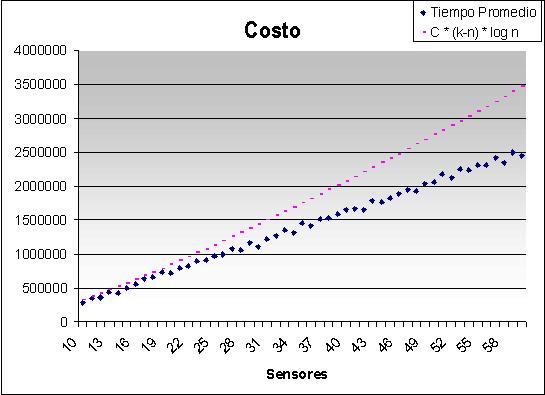
\includegraphics[scale=0.8]{ej2.jpg}
	\caption{ Se compara el tiempo que tard\'o en promedio en obtener un resultado contra el tiempo te\'orico del peor caso}
\end{figure}



\quad Armamos el test de la siguiente manera. Vamos a hacer instancias que vayan de 10 sensores a 100 y por cada cantidad de sensores realizamos 1000 repeticiones. Decidimos que la falla se produzca en la medici\'on: \quad $20 * n + r $. Donde n es la cantidad de sensores y r un valor aleatorio entre 1 y n.

\quad Para cada ejecuci\'on guardamos el tiempo que tard\'o usando la funci\'on \textit{clockgettime}


\subsection{Conclusiones}

\quad Como era de esperar, los resultados mostraron que el tiempo de ejecuci\'on es asint\'oticamente menor al tiempo te\'orico calculado para el peor caso. Siendo ese tiempo, menor al pedido por la consigna del trabajo pr\'actico.

\quad

\quad Analizar bien las posibles estructuras de datos a utilizar fue fundamental para volver m\'as eficiente el algoritmo. El problema de obtener en cada instante el m\'inimo de un conjunto de valores utilizando un minHeap logr\'o bajar la complejidad lineal a logar\'itmica.

\quad

\quad Luego, tambi\'en era necesario considerar la parte del problema en que todos los sensores realizan una medici\'on en el momento inicial. Lo que permite realizar n iteraciones menos de nuestro algoritmo, donde n es la cantidad de sensores.